\documentclass[10pt]{article}\usepackage[margin=.65in]{geometry}\usepackage[T1]{fontenc}\usepackage{graphicx}\setlength{\parindent}{0pt}\setlength{\parskip}{7pt}\sloppy\begin{document}{\large Isolated vertex insertion: owner, cardinality and forest invariants}\par Producer construction T-1332; publication T-1333. This packet models the completed-success path of SignedGraph::node at source revision 87fe3c0222. It extends the parent and owner maps by a new fixed point, gives the new vertex the identity potential, and pushes one onto the size array.\par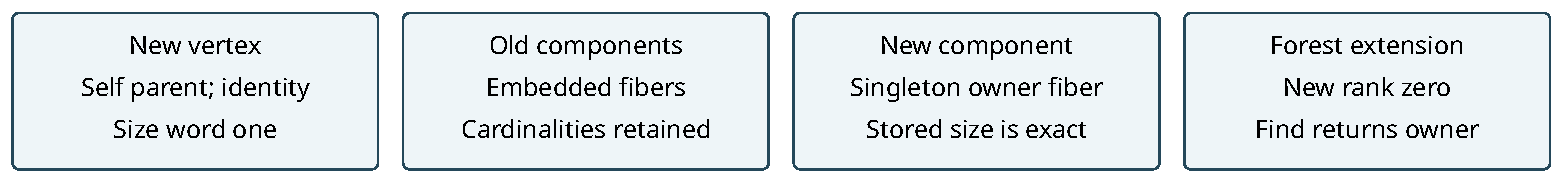
\includegraphics[width=\linewidth]{diagram.pdf}\par Result. Eleven named declarations compile. Existing owner fibers embed into the enlarged vertex type with unchanged cardinality; the new owner fiber is a singleton. The owner certificate and exact stored root-size cardinalities are preserved. Extending the forest rank by zero preserves the termination invariant, so a subsequent find still returns the certified owner for every old or new vertex.

Checks. Six controls compile: an old pair and old singleton keep their sizes, the inserted fiber has size one, the empty graph gains a singleton, the new owner differs from an old owner, and the new stored word is one. Seventeen separate named axiom readbacks contain only propext, Classical.choice and Quot.sound. Empty, renamed and sorryAx inventories are rejected. A deliberately false claim that the new singleton has cardinality two is rejected by Lean.

Assumptions and boundary. The initial graph already has the owner, root-size and forest invariants. This is a mathematical model of successful insertion; allocator failure and partial mutation during Vec pushes are not modeled. The parent/potential extension is functional, not yet a byte-level refinement of all four Rust vectors. Anchor insertion, signed semantic validity, counters and the complete native node/union path remain to be composed. The next-length condition n+1 $<$ USize.size retains the earlier union-size representability requirement; cardinality preservation itself needs no arithmetic-size premise.

Evidence. Each bounded module check uses one thread, 4096 MiB and a 120-second timeout, with source/dependency hashes before and after. Imported compiled dependencies are reused, not independently rebuilt. Pre/post hashes do not exclude transient edits. Two size-proof attempts, one premature dependent import, two control attempts and a declaration probe failed; all remain recorded separately from the deliberate false theorem. Independent source-fidelity review is pending. No scientific execution, timing, cohort change or budget renewal occurred.

Next construction. Connect the four native vector pushes, including the new None anchor, to the successful abstract insertion and prove preservation of signed equations and fixed-root truth. The previous component-size report remains an immutable historical snapshot; this packet supplies its previously pending owner/size/forest growth step.
\end{document}